\documentclass{article}
\usepackage[a4paper, margin=1in]{geometry} % Adjust margin size as needed
\usepackage{graphicx} % Required for inserting images
\usepackage{listings}
\lstset{basicstyle=\ttfamily}
\usepackage{float}
\usepackage{courier}
\usepackage{tabularx}
\usepackage{tikz}
\usepackage{url}
\usepackage{amsmath}
\usepackage{float}
\usepackage{hyperref}
\usepackage{MnSymbol}
\usepackage{indentfirst}

\title{Concepts of Programming - Project \#1: Chord Calculator}
\author{Daniel Marin and Jennifer Vicentes}
\date{October 22$^{nd}$, 2024}

\begin{document}
\maketitle
\tableofcontents
\newpage
\section{Introduction}
The purpose of this project was to put in practice de concepts seen in class, by creating a fully fledged chord calculator based on the subject of parsing primarily and the concepts of programming as a whole.
\subsection{Context}
For the 3$^{rd}$ deliverable of this project we where expected to create a chord calculator which is basically a pitch class description of each chord in a song. For the elaboration of this deliverable we used the code from the 2$^{nd}$ deliverable and modified it so as to be able to calculate the pitch class of each chord. As usual we used the grammar rules and the follow sets as the base for the creation of this project. 
\subsubsection{Grammar Rules}
\begin{figure}[H]
    \centering
    \begin{lstlisting}
      input:=  song EOF
       song:=  bar {bar} "|"
        bar:=  [meter] chords "|"
      meter:=  numerator "/" denominator
  numerator:=  "1" | "2" | "3" | ... | "15"
denominator:=  "1" | "2" | "4" | "8" | "16"
     chords:=  "NC" | "%" | chord {chord}
      chord:=  root [description] [bass]
       root:=  note
       note:=  letter [acc]
     letter:=  "A" | "B" | "C" | ... | "G" |
description:=  qual | qual qnum | qnum | qnum sus | sus
       qual:=  "-" | "+" | "o"
       qnum:=  ["^"] num
        num:=  "7" | "9" | "11" | "13"
        sus:=  "sus2" | "sus4"
       bass:=  "/" note
        acc:=  "b" | "#"
    \end{lstlisting}
    \caption{Chords Grammar. The input consists of the chords in a song separated by bar lines "$|$" plus optional meter information for the bars. (This grammar is a subset of the grammar used by Polynizer: \url{https://www.polynizer.com})}
    \label{fig:Grammar}
\end{figure} 
All grammar related functions in 'ChordCalc.c' are an interpretation of the grammar rules shown in figure \ref*{fig:Grammar}. With the use of the concepts seen in class and in the book. Also, as mentioned before here we have the first and follow sets of this grammar from deliverable one of this project.
\subsubsection{First and Follow Sets of Grammar}
\begin{figure}[H]
    \def\arraystretch{1.5}%
    \begin{tabularx}{\textwidth}{l|X|X}
        Nonterminal & First set & Follow set \\
        \hline
        \hline
        \lstinline|input| & \{1, 2, 3, 4, 5, \ldots, 15, \%, \texttt{NC}, A, B, C, D, E, F, G\} & \{\}\\
        \hline
        \lstinline|song| & \{1, 2, 3, 4, 5, \ldots, 15, \%, \texttt{NC}, A, B, C, D, E, F, G\} & \{\texttt{EOF}\}\\
        \hline
        \lstinline|bar| & \{1, 2, 3, 4, 5, \ldots, 15, \%, \texttt{NC}, A, B, C, D, E, F, G\} & \{ $\vert$, 1, 2, 3, 4, 5, \ldots, 15\} \\
        \hline
        \lstinline|meter| &  \{1, 2, 3, 4, 5, \ldots, 15\} 
        & \{\%, \texttt{NC}, A, B, C, D, E, F, G\} \\
        \hline
        \lstinline|numerator| & \{1, 2, 3, 4, 5, \ldots, 15\} 
        & \{ /\}\\
        \hline
        \lstinline|denominator| & \{1, 2, 4, 8, 16\} 
        & \{\%, \texttt{NC}, A, B, C, D, E, F, G\} \\
        \hline
        \lstinline|chords| & \{\%, \texttt{NC}, A, B, C, D, E, F, G\}
        & \{ $\vert$ \} \\
        \hline
        \lstinline|chord| & \{A, B, C, D, E, F, G\}  & 
        \{ $\vert$, A, B, C, D, E, F, G\} \\
        \hline
        \lstinline|root| & \{A, B, C, D, E, F, G\} 
        & \{-, +, o, \lstinline|^|, 7, 9, 11, 13, \texttt{sus2}, \texttt{sus4}, /, $\vert$, A, B, C, D, E, F, G\} \\
        \hline
        \lstinline|note| & \{A, B, C, D, E, F, G\} 
        & \{-, +, o, \lstinline|^|, 7, 9, 11, 13, \texttt{sus2}, \texttt{sus4}, /, $\vert$, A, B, C, D, E, F, G\} \\
        \hline
        \lstinline|letter| & \{A, B, C, D, E, F, G\} 
        & \{\#, b, -, +, o, \lstinline|^|, 7, 9, 11, 13, \texttt{sus2}, \texttt{sus4}, /, $\vert$, A, B, C, D, E, F, G\} \\
        \hline
        \lstinline|description| & \{-, +, o, \lstinline|^|, 7, 9, 11, 13, \texttt{sus2}, \texttt{sus4}\}  & \{/, $\vert$, A, B, C, D, E, F, G\} \\
        \hline
        \lstinline|qual| & \{-, +, o\} 
        & \{/, $\vert$, A, B, C, D, E, F, G,\lstinline|^|, 7, 9, 11, 13\} \\
        \hline
        \lstinline|qnum| & \{\lstinline|^|, 7, 9, 11, 13\}  & \{/, $\vert$, A, B, C, D, E, F, G, \texttt{sus2}, \texttt{sus4}\}  \\
        \hline
        \lstinline|num| & \{7, 9, 11, 13\} 
        & \{/, $\vert$, A, B, C, D, E, F, G, \texttt{sus2}, \texttt{sus4}\} \\
        \hline
        \lstinline|sus| & \{\texttt{sus2}, \texttt{sus4}\} 
        & \{/, $\vert$, A, B, C, D, E, F, G\}  \\
        \hline
        \lstinline|bass| & \{/\} 
        & \{ $\vert$, A, B, C, D, E, F, G\}\\
        \hline
        \lstinline|acc| & \{\#, b\} 
        & \{-, +, o, \lstinline|^|, 7, 9, 11, 13, \texttt{sus2}, \texttt{sus4}, /, $\vert$, A, B, C, D, E, F, G\} \\
        \hline
    \end{tabularx}
    \caption{First and Follow Sets of the Grammar in figure \ref*{fig:Grammar} developed in deliverable 1.}
    \label{fig:FirstAndFollowSets}
\end{figure}
Figure \ref*{fig:Grammar} and \ref*{fig:FirstAndFollowSets} helped us develop the flow of the program and it's elaboration in a concise but proper manner. This report document focuses on explaining each function, the tests that where performed to prove functionality.
\subsection{Usage}
The program developed for this deliverable is named 'ChordCalc.c', to use this program you must first have the '.txt' file in a folder (preferrebly the songs folder). Run the program, when prompeted "\texttt{Enter the path of the file to be parsed:}" copy the file path. The outputs would appear as follows:
\begin{figure}[H]
    \begin{lstlisting}
        4/4 Db^7 Ab/C C+7 | F-11 Bb9 | Eb9sus4 | Eb13sus4 Eb13 ||  
    \end{lstlisting}
    \caption{Sample input '.txt' contents consisting of the introductory chords of \textit{El dia que me quieras} by Carlos Gardel and Alfredo Le Pera (version by Luis Miguel)}
    \label{fig:SampleInput}
\end{figure}
\begin{figure}[H]
    \begin{lstlisting}
                    0  1  2  3  4  5  6  7  8  9  A  B
                    -  -  -  -  -  -  -  -  -  -  -  -
                1.  *  *           *        *          - Db^7
                2.  *        *              *          - Ab/C
                3.  *           *           *     *    - C+7
                4.  *        *     *        *     *    - F-11
                5.  *     *        *        *     *    - Bb9
                6.     *     *     *        *     *    - Eb9sus4
                7.  *  *     *              *     *    - Eb13sus4
                8.  *  *     *           *        *    - Eb13
                    -  -  -  -  -  -  -  -  -  -  -  - 
                    7  4  1  5  1  4  0  1  7  0  6  0
    \end{lstlisting}
    \caption{Format for the output. Showing the pitch class number as the header of a table and marking with stars the notes that make up the chords, where A = 10 and B = 11. At the end of document we have the totals.}
    \label{fig:SampleOutput}
\end{figure}
\subsection{Platform}
The development of this project was all done in C with the help of the grammar rules and Chapter 6.6 - Parsing Techniques and Tools from Programming Languages - Kenneth C. Louden - 3ed.
\section{Data Structures}
Two data stuctures where used to develop this program, the \texttt{Chord} which repersents the values of individual Chords being parsed. With these two data structures we managed to create the logic of the Chord Calculator accordingly. The chord data structure is of the format:
\begin{lstlisting}
            typedef struct {
                char root[3];       // D, Db or D#
                char qual;          // -, +, o, none 
                int sus;            // sus2 or sus4
                char ext_type;      // ^ or none 
                int extension;      // 7, 9, 11, 13
                char bass[3];       // D, Cb or C
            } Chord;
\end{lstlisting}
Also, we utilized the linked list data structure to dynamically hold a list of chords that gets created as we parse the current .txt file, which is of form:
\begin{lstlisting}
                    typedef struct ChordNode {
                        Chord chord;
                        struct ChordNode* next;
                    } ChordNode;
\end{lstlisting}
\section{Functions} \label{fig:Functions}
\subsection{Main}
The main function is in charge of the logic behind coordinating the functions to parsing and printing, and the file retrival. The code behind this function is:
\begin{figure}[H]
    \begin{lstlisting}[language=C]
int main(void) {
    char filepath[365];
    printf("Enter the path of the file to be parsed: ");
    scanf("%[^\n]s", filepath);
    if (strlen(filepath) < 4 || 
        strcmp(filepath + strlen(filepath) - 4, ".txt") != 0) {
        printf("Error: Only .txt files are supported\n");
        exit(1);
    }
    inputFile = fopen(filepath, "r");
    if (inputFile == NULL){
        printf("Error: cannot open file\n");
        exit(1);
    }
    printf("The following characters demonstrate the tokens being parsed.\n\n");
    getToken();
    input();
    printf("\n");
    printf("\nParsing completed successfully\n");
    fclose(inputFile);
    return 0;
}
    \end{lstlisting}
    \caption{Uncommented \texttt{main} function in charge of coordinating the parsing, printing and file retrieving for this program.}
    \label{fig:MainFunc}
\end{figure}
As demonstrated in the section of code from above, this function follows a set of steps to properly coordinate the behavior of the Chord Calculator:
\begin{itemize}
    \item Getting the filepath from the user.
    \item Checking if the file is supported and if it can be opened.
    \item Parse the contents of the program.
\end{itemize}
\subsection{Token Validation}
The functions in this section are in charge of retrieving tokens, checking if the token is what is expected, and prompting error messages when needed. 
\subsubsection{\texttt{void error(char *message)}}
This function is at simple as it gets, whenever called it is supposed to print out a message for the user to see whenever there is an error parsing, and exit the program. In this program it is primarily used to catch parsing errors and prevent them from propagating later on.
\begin{figure}[H]
    \begin{lstlisting}[language=C]
void error(char* message) {
    printf("\nParse error: %s\n", message);
    exit(1);
}
    \end{lstlisting}
    \caption{Uncommented \texttt{error} function from Parser.c}
\end{figure}
\subsubsection{\texttt{void getToken()}}
This function is in charge of retrieving the next token to be parsed whenever it is called, ignoring newlines, tabulars and spaces. Thus retrieving possibly parsable tokens from the file. This function is based on what was seen in class.
\begin{figure}[H]
    \begin{lstlisting}[language=C]
void getToken(){
    token = getc(inputFile);
    if (token == EOF) return; 
    while(token == ' ' || token == '\n' || token == '\t'){
        token = getc(inputFile);
    }
}
    \end{lstlisting}
    \caption{Uncommented \texttt{getToken} function from Parser.c}
\end{figure}
\subsubsection{\texttt{void match(char c, char* message)}} 
This function is a controller that is in charge of deciding whether the current token is the desired character and we should prompt the \texttt{getToken()} function to continue parsing, or if there was an error parsing and it should prompt an \texttt{error(message)}.
\begin{figure}[H]
    \begin{lstlisting}[language=C]
void match(char c, char* message){
    if (token == c) 
        getToken();
    else 
        error(message);
}
    \end{lstlisting}
    \caption{Uncommented \texttt{match} function from Parser.c}
\end{figure}
\subsection{Grammar Functions}
The functions in this section are based on the grammar rules seen in figure \ref{fig:Grammar}, which define the rules in which the parsing should take place. They are fairly similar to the functions from deliverable 2, but with the added functionality that when parsing they create a list of chords.
\subsubsection{\texttt{void input()}}
This function is in charge of initializing the parsing and the list of chords (linked list), calling the match, finalize the parsing by matching the \texttt{EOF} character at the end of the file. Once the parsing takes place, this function prints out the Chords in the format stated by figure \ref{fig:SampleOutput} before freeing the list of chords.
\subsubsection{\texttt{void song(ChordNode** head)}}
This function is in charge of parsing the structure of the song, by parsing bars until it encounters a \texttt{|} after any bar, insinuating that the song has ended, with the added functionality of passing the pointer to bar as to record the chords being played.
\subsubsection{\texttt{void bar(ChordNode** head)}}
This function is in charge of parsing the structure of a bar, checking for the optional meter by checking if the current token is a digit, calling the chords method, and finally matching the end of a bar with the \texttt{|} char.
\subsubsection{\texttt{void meter()}}
This function is in charge of parsing the structure of a meter, first retrieving a numerator, matching the '/' and finally retrieving the denominator.
\subsubsection{\texttt{int numerator()}}
This function is in charge of checking if the numerator is in the valid range (from 1 - 15), and then returning if valid. Else, it should prompt an error. 
\subsubsection{\texttt{int denominator()}}
This function is in charge of checking if the denominator is a valid one (denominator $\in$ [1,2,4,8,16]), and returning if so. Else, it should prompt an error.
\subsubsection{\texttt{void chords(ChordNode** head)}}
This function is in charge of parsing the structure of a set of chords by either matching the characters \texttt{NC} or \texttt{\%}, or checking for a repeated set of chords. It has the added functionality of passing the head of the list to the chord function for it to register the current chord it is parsing. 
\subsubsection{\texttt{void chord(Chord* chord)}}
This function is in charge of parsing the structure of a chord by retrieving the root, checking if the chord has a description and a bass and parsing the chord accordingly. It also, appends each chord to the list of chords whenever parsing of the chord has been completed.
\subsubsection{\texttt{void root(char* root)}}
This function is charge of calling note and is used to separate the logic of the root from the bass which represent different parts of the same chord. 
\subsubsection{\texttt{void note(char* res)}}
This function is in charge of parsing the structure of a note by calling \texttt{letter} function and then checking if it should call the \texttt{acc} function, it then places those results in the correct position of the chord data structure.
\subsubsection{\texttt{char letter()}}
This function is in charge of checking if the letter is in the range from A to G, and returing it for the note to store it if it is in the range.
\subsubsection{\texttt{char acc()}}
This function is in charge of checking if the accent is a valid one (either \# or b), and returning it to the note to store.
\subsubsection{\texttt{void description(Chord* chord)}}
This function is in charge of checking which of the optional description rules is being used by the chord, by using a dedicated set of valid combinations seen in this rule, and then storing the information of the chord.
\subsubsection{\texttt{char qual()}}
This function is in charge of checking if the quality of the chord is a valid one, and returning which quality it is to the description.
\subsubsection{\texttt{void qnum(Chord* chord)}}
This function is in charge of checking for valid combinations of a qnum and a num (options are a \texttt{\^{}} symbol and a num or a num), and saving this information accordingly.
\subsubsection{\texttt{int num()}}
This function is in charge of checking using the same method as the numerator for a valid number $\in$ [7,9,11,13]. This returns it also or prompts an error.
\subsubsection{\texttt{void sus(Chord* chord)}}
This function is in charge of is in charge of checking if the suspension is either $sus2$ or $sus4$, and saving it in the chord.
\subsubsection{\texttt{void bass(char* bass)}}
This function is in charge  is in charge of parsing the structure of a bass by matching the '/' and prompting the \texttt{note} function, and storing the results of the note into the bass section of the chord.

\subsection{Chord Calculator Functions}
\subsubsection{\texttt{ChordNode* createNode(Chord chord)}} This function allocates memory for a new \texttt{ChordNode} containing the provided chord data. It initializes the node with the chord data and sets its \texttt{next} pointer to \texttt{NULL}. If memory allocation fails, an error message is displayed, and the program exits.

\subsubsection{\texttt{ChordNode* appendChord(ChordNode* head, Chord chord)}} This function appends a new chord to the end of the linked list of chords. If the list is empty, the new node becomes the head. Otherwise, it traverses to the end of the list and links the new node there to maintain the order of printing.

\subsubsection{\texttt{void printChords(ChordNode* head)}} This function traverses the linked list, printing each chord's pitch class and description. It also maintains a tally of pitch class occurrences for each chord and displays a summary of counts after listing all chords.

\subsubsection{\texttt{void createChordArr(Chord* chord, int* arr)}} This function creates a pitch class array for a chord by marking notes based on the chord's root, quality, extension, and bass. The array is updated based on the chord's characteristics to represent pitch classes on a 12-tone scale.

\subsubsection{\texttt{int noteToPitchClass(const char* root)}} This function converts a root note into its corresponding pitch class (0-11). It accounts for accidentals (\texttt{b} and \texttt{\#}) and returns -1 if the note is invalid.

\subsubsection{\texttt{void printChord(Chord* chord)}} This function prints the chord's root, quality, extension, suspension, and bass. It formats the chord's attributes into a readable representation, including any extensions, suspensions, or bass notes.

\subsubsection{\texttt{void freeChords(ChordNode* head)}} This function deallocates memory for each node in the chord linked list, preventing memory leaks by iterating through the list and freeing each node individually.
\section{Test and Results} \label{fig:Results}
The test for the program are all the '.txt' files posted by Dr. Arturo Camacho on blackboard and the sample input .txt, they are songs parsed using Polynizer app\footnote{Polynizer app link: \url{https://www.polynizer.com}} which are just a set of terminals/tokens bundled in a neatly organized manner, that when played create a song. The format of these results are as follows, only the last few chords and the total times each pitch class is played will be in this document.
\begin{figure}[H]
    \centering
    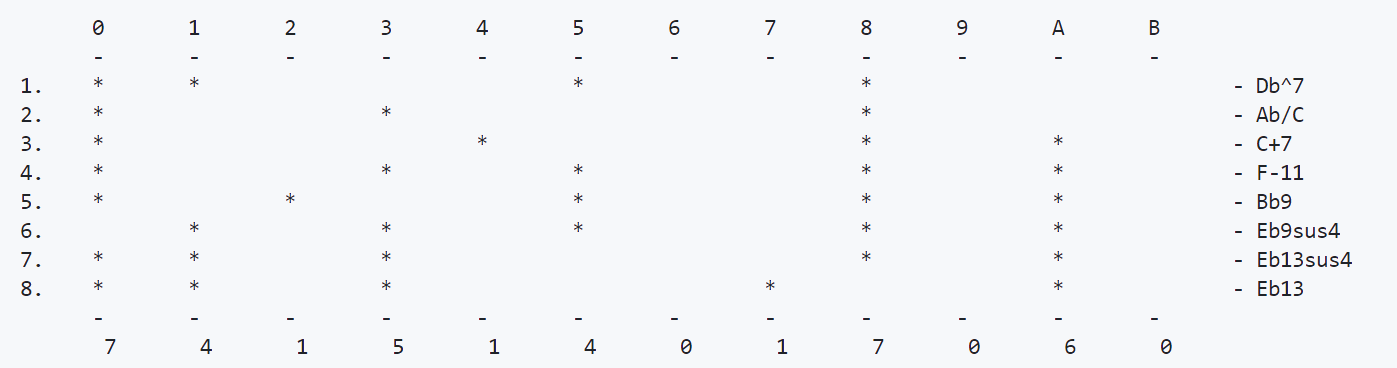
\includegraphics[width=1\textwidth]{Image_SampleOutput.png}
    \caption{Test and Results Format}
\end{figure}
Those tests are encompassed by the following itemize, which are the files in the Songs folder and their respective results. 
\begin{itemize}
    \item \textbf{Test 1}: Bruno Mars, Anderson Paak, Silk Sonic - Skate.txt
    \begin{figure}[H]
        \centering
        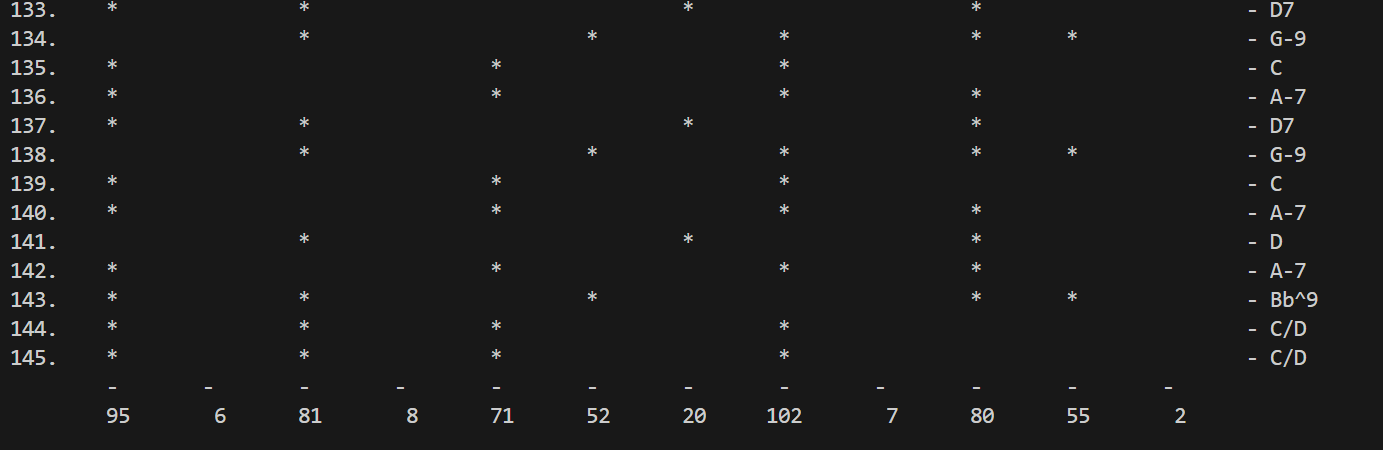
\includegraphics[width=1\textwidth]{Image_SkateParsed.png}
        \caption{Image of outputs on the command line.}
    \end{figure}
    \item \textbf{Test 2}: John Legend - All of me.txt
    \begin{figure}[H]
        \centering
        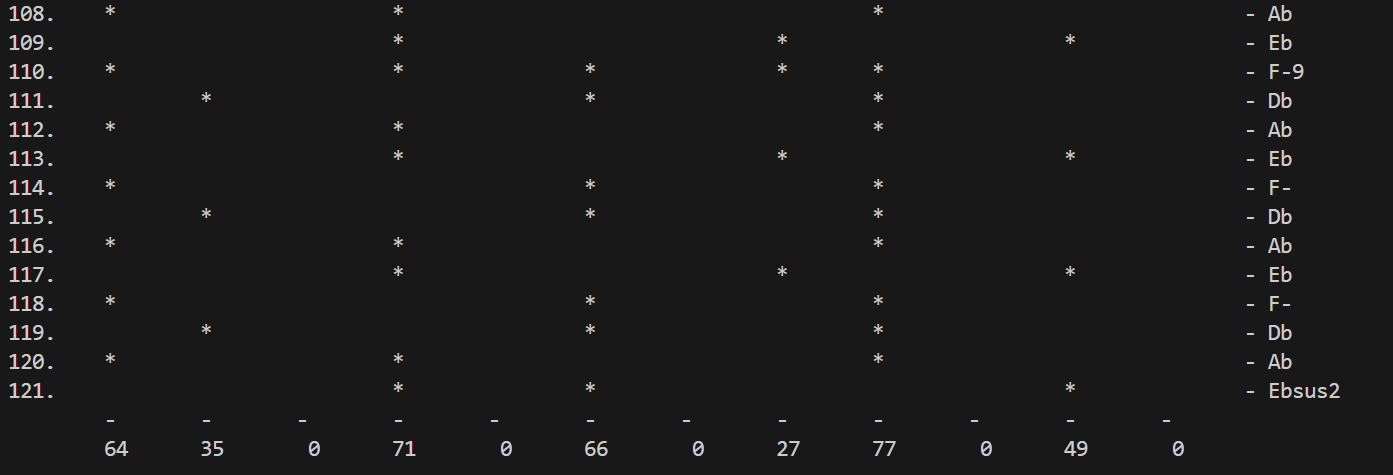
\includegraphics[width=1\textwidth]{Image_AllOfMeParsed.png}
        \caption{Image of outputs on the command line.}
    \end{figure}
    \item \textbf{Test 3}: Luis Miguel - El dia que me quieras.txt
    \begin{figure}[H]
        \centering
        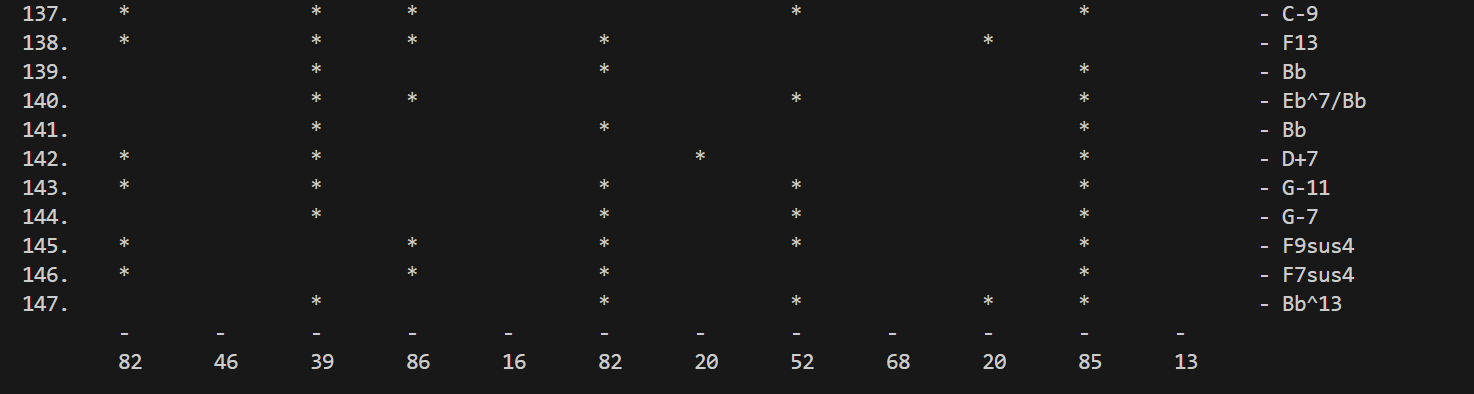
\includegraphics[width=1\textwidth]{Image_ElDiaQueMeQuiera.png}
        \caption{Image of outputs on the command line.}
    \end{figure}
    \item \textbf{Test 4}: Paul McCartney - Uncle Albert / Admiral Halsey (medley).txt
    \begin{figure}[H]
        \centering
        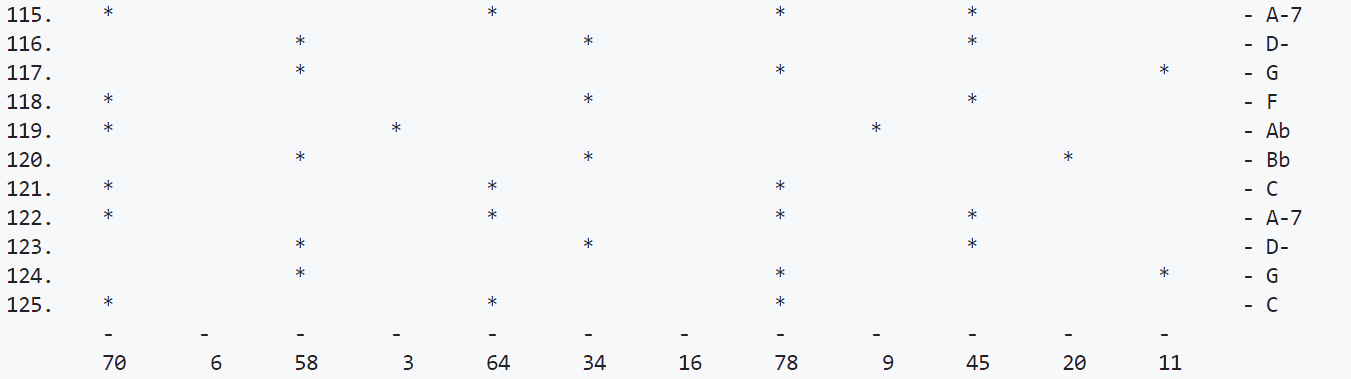
\includegraphics[width=1\textwidth]{Image_AdmiralHalsey.png}
        \caption{Image of outputs on the command line.}
    \end{figure}
    \item \textbf{Test 5}: Queen - Don't stop me now.txt
    \begin{figure}[H]
        \centering
        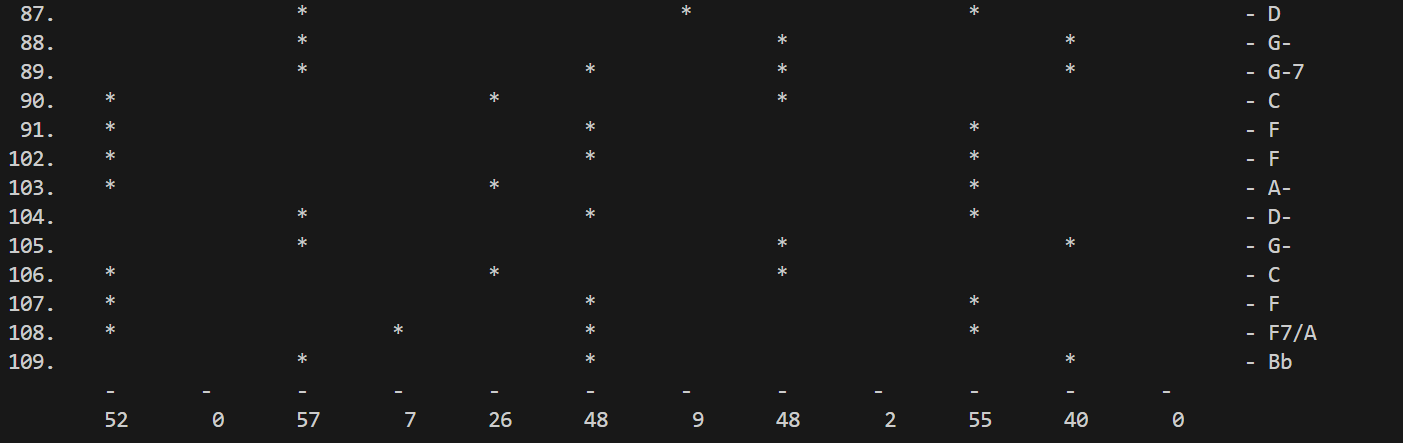
\includegraphics[width=1\textwidth]{Image_DontStopMeNow.png}
        \caption{Image of outputs on the command line.}
    \end{figure}
    \item \textbf{Test 6}: Rocio Durcal - La gata bajo la lluvia.txt
    \begin{figure}[H]
        \centering
        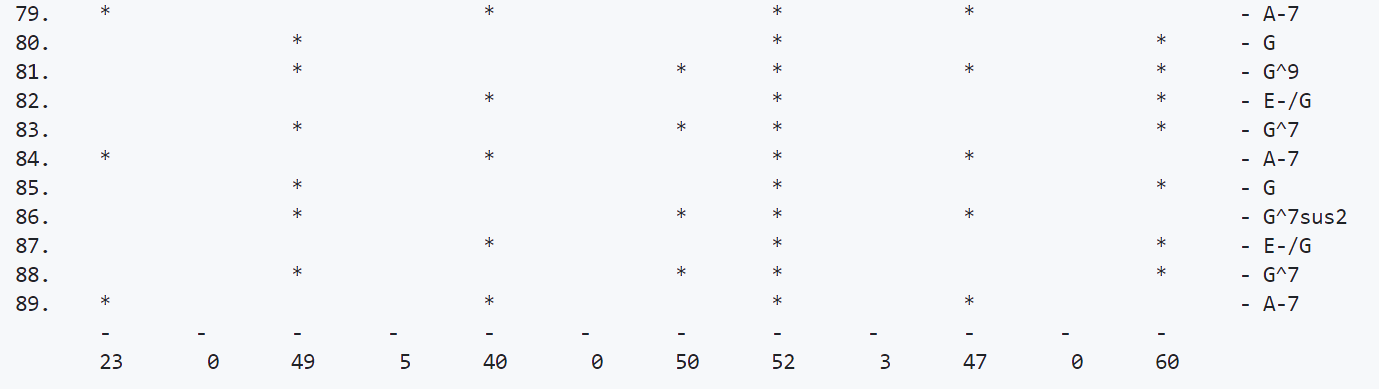
\includegraphics[width=1\textwidth]{Image_LaGataBajoLaLluvia.png}
        \caption{Image of outputs on the command line.}
    \end{figure}
    \item \textbf{Test 7}: Soda Stereo - The musica ligera.txt
    \begin{figure}[H]
        \centering
        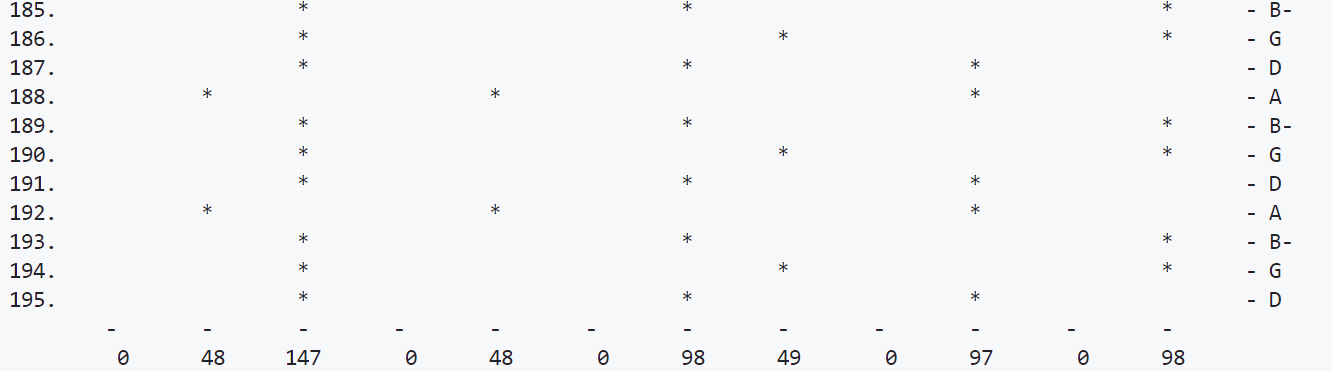
\includegraphics[width=1\textwidth]{Image_DeMusicaLigeraParsed.png}
        \caption{Image of outputs on the command line.}
    \end{figure}
\end{itemize}
\section{Discussion}
This deliverable manages to encompass the desire behavior of the chord calculator. It manages to do so with the use of the functions seen in section \ref{fig:Functions}, with proven results in Section \ref{fig:Results} with the use of the examples sent by the professor. The examples are in the folder \textbf{Songs} appended with this document. For a more detailed analysis on the functions used to develop the overall functionality please revise the \textbf{ChordCalc.c} file found in the same folder as this document.
\end{document}